\section{本章小结}

至此,时域上的分析方法都已介绍完毕。
系统在时域本质上就是回响的混响,所以时域模型就是研究回响和混响。

\begin{figure}[h]
\centering
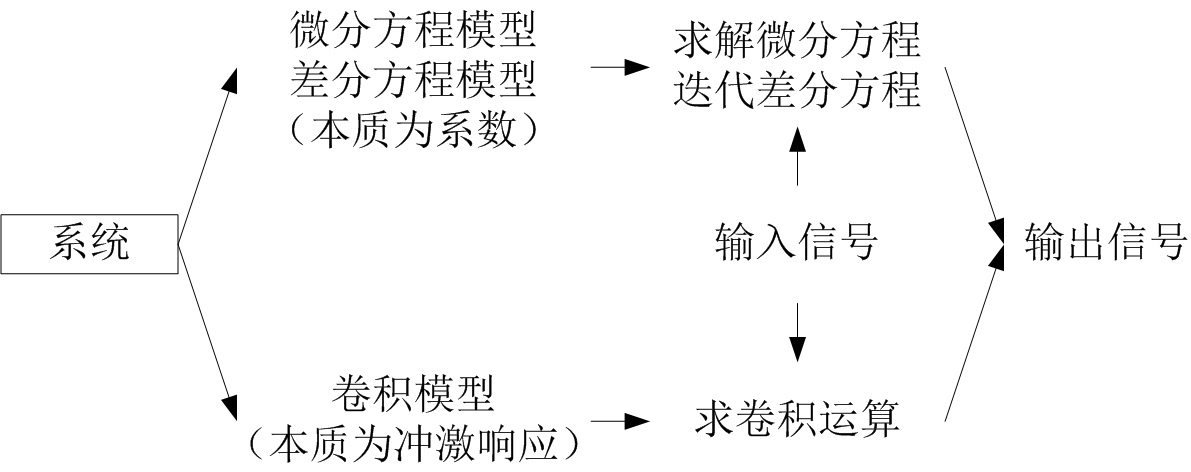
\includegraphics[height=4cm]{3.4-1.png}
\end{figure}

时域分析的目的是在已知输入的情况下求解系统的输出。
为此,需要两个步骤:1)建立系统模型,2)对于给定输入计算输出。

系统的两种时域模型:
\begin{itemize}
    \item 微分/差分方程:系数表示系统回响,微分方程表示系统混响,难在求解微分方程;
    \item 卷积:冲激响应表示回响,卷积运算表示混响,难在获得系统的冲激响应,注意冲激响应描述的是系统对冲激函数的响应,而非输入输出关系。
\end{itemize}

有了模型之后,求解输出:
\begin{itemize}
    \item 微分/差分方程:将输入信号带入方程求解输出的解析解,或用迭代法求解输出信号的数值序列;
    \item 卷积:将输入信号和冲激响应作卷积运算,获得输出信号。
\end{itemize}




